Dopo una prima applicazione dei filtri sopra descritti, si passa all’applicazione di un threshold tramite la funzione \texttt{cv2.threshold} della libreria OpenCV. Il suo funzionamento è semplice: essa prende in input un’immagine in grayscale ed effettua un confronto tra i valori dei singoli pixels e un valore di soglia. Considerando un caso binario, se il valore di un pixel è maggiore del valore di soglia, viene assegnato un valore specifico al pixel stesso (bianco o nero), altrimenti viene assegnato il valore opposto.

\begin{minted}
  [
    xleftmargin=\parindent,
    framesep=2mm,
    baselinestretch=1.2,  
    fontsize=\footnotesize,
    linenos,
    breaklines
  ]
  {python}
  
  def threshold(img, tValue, adaptive=False, binaryInv=False, otsu=False, dilate=False):
    if adaptive is False and otsu is False:
        _, thresh = cv2.threshold(img, tValue,
                                  255, cv2.THRESH_BINARY_INV if binaryInv else cv2.THRESH_BINARY)
    elif adaptive is True and otsu is False:
        thresh = cv2.adaptiveThreshold(
            img, 255, cv2.ADAPTIVE_THRESH_MEAN_C, cv2.THRESH_BINARY, 9, 1)
    elif adaptive is False and otsu is True:
        ret, thresh = cv2.threshold(
            img, 0, 255, cv2.THRESH_BINARY_INV + cv2.THRESH_OTSU)
    else:
        thresh = img

    if dilate is True:
        thresh = dilate_thresh(thresh)

    return thresh
    
\end{minted}

La funzione applica diversi threshold in base ai parametri scelti; nel caso dell’identificazione dell’iride si è scelto di applicare un threshold binario (default della funzione) all’immagine filtrata, il quale assegna ad un pixel il valore 255 (bianco) se il valore attualmente presente nel pixel è maggiore della soglia identificata dal parametro tValue. Per il caso in esame il valore di soglia ottimale è risultato essere 160.

\begin{figure}[h]
  \centering
  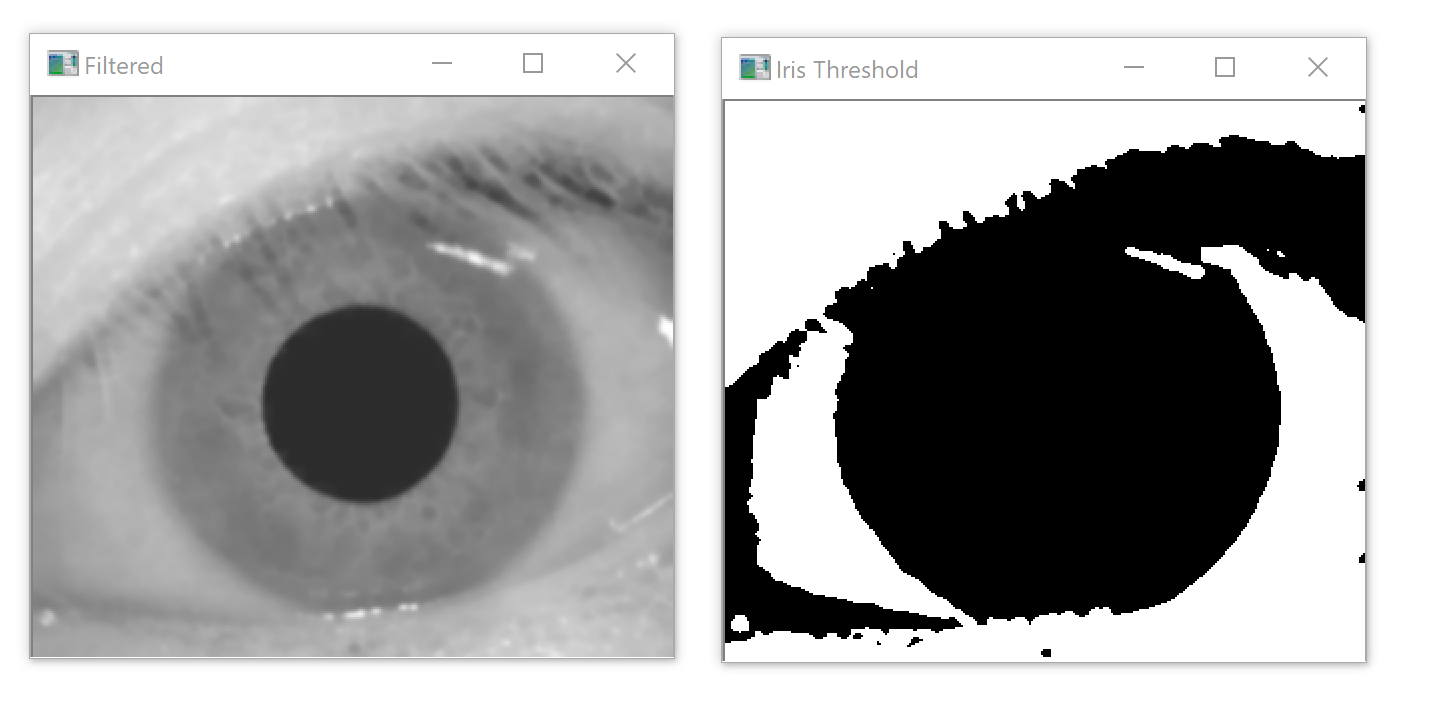
\includegraphics[width=1.0\textwidth]{threshold_iris.png}
  \caption{Applicazione del threshold binario per la delineazione dell'iride}
\end{figure}

Grazie a questo tipo di elaborazione si mette in risalto l’area dell’iride in modo da facilitare ulteriormente il successivo riconoscimento della circonferenza. 

Per il riconoscimento della pupilla si è utilizzato invece  un approccio simile, invece di applicare un classico threshold binario si è scelto di usare un threshold binario invertito, abilitando il parametro \texttt{BINARY\_INV}. L’unica differenza rispetto al threshold normale è che viene assegnato il valore 255 ai pixel minori del valore di soglia. La scelta è stata fatta perchè è risultato più performante utilizzare questo tipo di threshold per identificare l’area della pupilla, composta da pixel il cui valore di colore si avvicina di più allo 0 (nero). Il valore di soglia ottimale è risultato essere 70.

\begin{figure}[h]
  \centering
  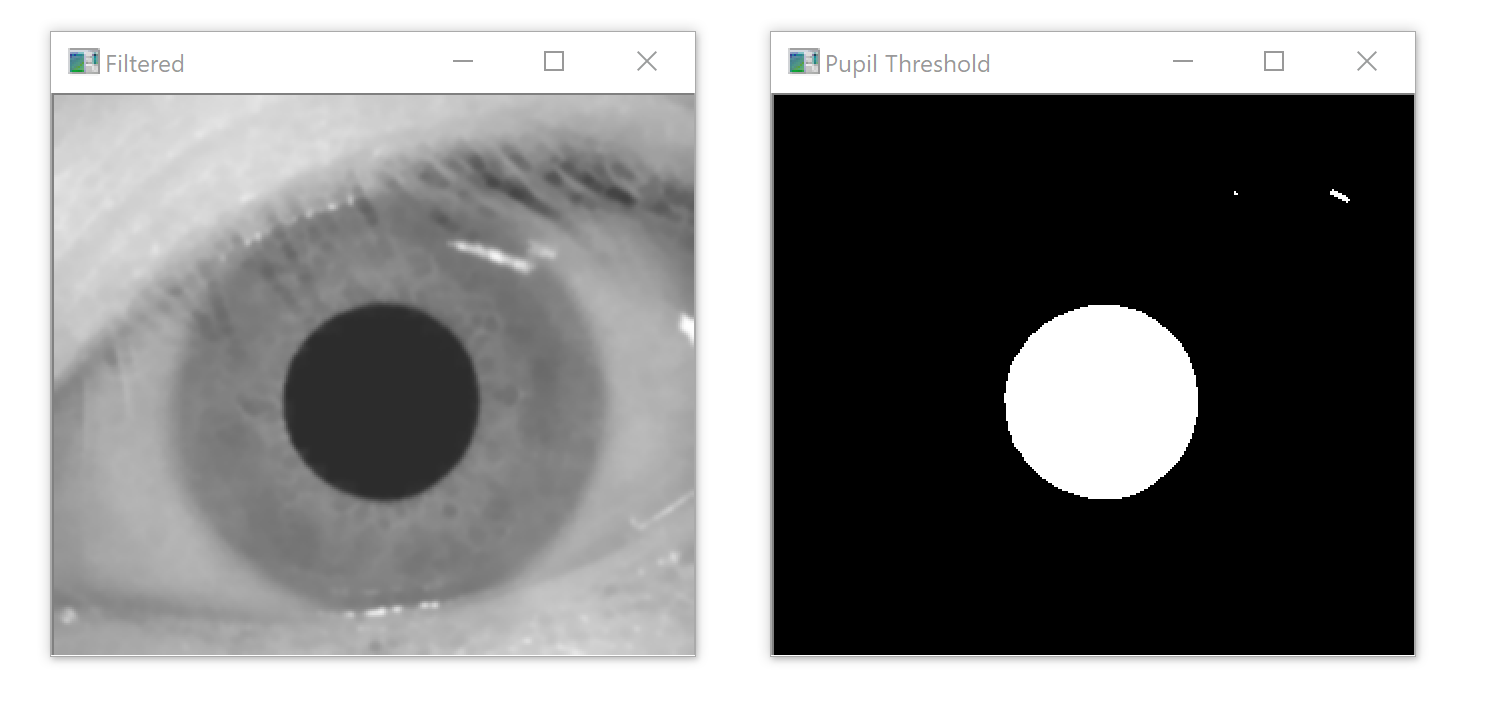
\includegraphics[width=1.0\textwidth]{threshold_pupil.png}
  \caption{Applicazione del threshold binario invertito per la delineazione della pupilla}
\end{figure}

La funzione di cui sopra prevede anche l’utilizzo di threshold diversi in base allo specifico impiego, essi sono attivabili modificando i relativi parametri presenti nelle sezioni \texttt{THRESHOLD\_PUPIL} e \texttt{THRESHOLD\_IRIS} del file di configurazione:

\begin{itemize}
  \item \textbf{Adaptive Threshold}: l’algoritmo calcola il threshold analizzando piccole regioni dell’immagine, ottenendo quindi diversi valori di soglia per diverse regioni. Si utilizza per immagini ad alto contrasto
  \item \textbf{Otsu Threshold}: l’algoritmo calcola in automatico il valore di soglia ottimale sulla base dell’istogramma dell'immagine
  \item \textbf{Dilate Threshold}: applica una trasformazione morfologica di dilatazione all’immagine ottenuta da una delle metodologie precedenti. L’utilità sarebbe quella di “riempire” i buchi
\end{itemize}

Nonostante fossero implementate tecniche di thresholding più avanzate, come Adaptive e Otsu, si è rivelato ottimale utilizzare il threshold binario normale e binario invertito in quanto gli algoritmi di identificazione di iride e pupilla si basano sul riconoscimento di cerchi nelle immagini, infatti con queste trasformazioni si vanno ad evidenziare maggiormente i cerchi delineati dall’iride e dalla pupilla.
